\documentclass{standalone}
\usepackage[utf8]{inputenc}
\usepackage{tikz}
\usepackage{lipsum}
\usepackage{mwe}
\usetikzlibrary{decorations.pathreplacing}
\begin{document}

\hspace{1cm}
\centering
\begin{minipage}[c]{1.775\textwidth}
\paragraph{ }
\paragraph{ }
\paragraph{ }

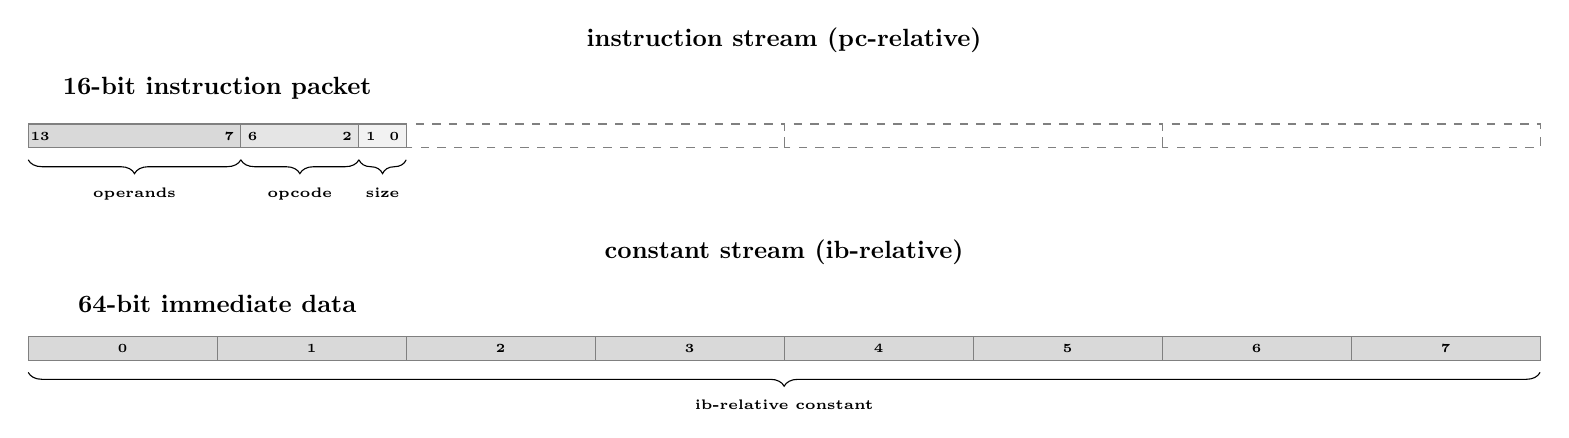
\begin{tikzpicture}[fill=blue!20,scale=0.3]
\begin{scope}[every node/.style={font=\normalsize, inner sep=0pt, right}]

\node [above,scale=0.9,anchor=south] at (32,4)  {\textbf{instruction stream (pc-relative)}};
\node [above,scale=0.9,anchor=south] at (8,2)  {\textbf{16-bit instruction packet}};

\fill [black!15] (0,0)    rectangle (9,1);
\draw [black!50] (0,0)    rectangle (9,1);
\node [font=\tiny,below,scale=0.9,anchor=north] at (0.5,0.66)  {$\textbf{13}$};
\node [font=\tiny,below,scale=0.9,anchor=north] at (8.5,0.66)  {$\textbf{7}$};

\fill [black!10] (9,0)     rectangle (14,1);
\draw [black!50] (9,0)     rectangle (14,1);
\node [font=\tiny,below,scale=0.9,anchor=north] at (9.5,0.66)  {$\textbf{6}$};
\node [font=\tiny,below,scale=0.9,anchor=north] at (13.5,0.66)  {$\textbf{2}$};

\fill [black!5] (14,0)     rectangle (16,1);
\draw [black!50] (14,0)     rectangle (16,1);
\node [font=\tiny,below,scale=0.9,anchor=north] at (14.5,0.66)  {$\textbf{1}$};
\node [font=\tiny,below,scale=0.9,anchor=north] at (15.5,0.66)  {$\textbf{0}$};

\draw [black!50,dashed] (16,0)     rectangle (32,1);
\draw [black!50,dashed] (32,0)     rectangle (48,1);
\draw [black!50,dashed] (48,0)     rectangle (64,1);

\draw [decorate,decoration={brace,amplitude=5pt,mirror,raise=4ex}]
    (0,1.5) -- (9,1.5) node[font=\tiny,midway,below,yshift=-2.7em]{\textbf{operands}};

\draw [decorate,decoration={brace,amplitude=5pt,mirror,raise=4ex}]
    (9,1.5) -- (14,1.5) node[font=\tiny,midway,below,yshift=-2.7em]{\textbf{opcode}};

\draw [decorate,decoration={brace,amplitude=5pt,mirror,raise=4ex}]
    (14,1.5) -- (16,1.5) node[font=\tiny,midway,below,yshift=-2.7em]{\textbf{size}};

\node [above,scale=0.9,anchor=south] at (32,-5)  {\textbf{constant stream (ib-relative)}};
\node [above,scale=0.9,anchor=south] at (8,-7)  {\textbf{64-bit immediate data}};

\foreach \x in {0,1,2,3,4,5,6,7}
  \fill [black!15] (\x*8,-9)    rectangle (\x*8+8,-8);

\foreach \x in {0,1,2,3,4,5,6,7}
  \draw [black!50] (\x*8,-9)     rectangle (\x*8+8,-8);

\foreach \x in {0,1,2,3,4,5,6,7}
  \node [font=\tiny,below,scale=0.9,anchor=north] at (\x*8 + 4,-8.33)  {$\textbf{\x}$};

\draw [decorate,decoration={brace,amplitude=5pt,mirror,raise=4ex}]
    (0,-7.5) -- (64,-7.5) node[font=\tiny,midway,below,yshift=-2.7em]{\textbf{ib-relative constant}};

\end{scope}
\end{tikzpicture}

\bigskip
\end{minipage}

\end{document}
